\chapter{QEF Calculation using the Eigen Library} \label{Chapter5}

The Quadratic Error Function is a mathematical formulation that minimizes the error in approximating data points. In the context of isosurface extraction, the QEF is employed to find the optimal position of a vertex within a cell. The Eigen library, a C++ template library for linear algebra, is utilized to compute the QEF point efficiently. Eigen provides the necessary tools to compute the Quadratic Error Function, which is pivotal in the Dual Contouring process (\cite{Eigen_2013}).

\section{Simplification of QEF Equation}

The Quadratic Error Function, while powerful, can be represented in a more concise and computationally efficient manner, especially when dealing with large datasets or real-time applications. By transforming the QEF into a matrix form, we can leverage the capabilities of linear algebra libraries, such as Eigen, to solve it more efficiently. This section delves into the process of simplifying the QEF equation, making it more amenable to computational methods and setting the stage for its application in isosurface extraction.

The formulation of the Quadratic Error Function and its matrix representation, as presented in Equations \ref{eq:qef_1}, \ref{eq:qef_2}, \ref{eq:qef_3} and \ref{eq:qef_4} are derived from the work of \cite{Ju_2002}. 

\begin{equation}
E[\mathbf{x}] = \sum_{i} \left( \mathbf{n}_i \cdot (\mathbf{x} - \mathbf{p}_i) \right)^2
\label{eq:qef_1}
\end{equation}

\noindent where \( \mathbf{n}_i \) are the normals, \( \mathbf{p}_i \) are the positions, and \( \mathbf{x} \) is the point which minimizes this error function. The QEF can be rewritten in matrix form as:

\begin{equation}
E[\mathbf{x}] = (\mathbf{Ax} - \mathbf{b})^T (\mathbf{Ax} - \mathbf{b})
\label{eq:qef_2}
\end{equation}

\noindent where \( \mathbf{A} \) is a matrix whose rows are the normals \( \mathbf{n}_i \), and \( \mathbf{b} \) is a vector whose elements are \( \mathbf{n}_i \cdot \mathbf{p}_i \). It can be expanded further into the following form.

\begin{equation}
E[\mathbf{x}] = \mathbf{x}^T \mathbf{A}^T \mathbf{A} \mathbf{x} - 2 \mathbf{x}^T \mathbf{A}^T \mathbf{b} + \mathbf{b}^T \mathbf{b}
\label{eq:qef_3}
\end{equation}

\noindent In this representation (Equation \ref{eq:qef_3}), the matrix \( \mathbf{A}^T \mathbf{A} \) is a symmetric \( 3 \times 3 \) matrix, while \( \mathbf{A}^T \mathbf{b} \) is a column vector with three elements, and \( \mathbf{b}^T \mathbf{b} \) is a scalar value. A primary benefit of this expanded form is the reduced storage requirement: only the matrices \( \mathbf{A}^T \mathbf{A} \), \( \mathbf{A}^T \mathbf{b} \), and the scalar \( \mathbf{b}^T \mathbf{b} \) need to be retained, amounting to just 10 floating-point values. This is in contrast to retaining the entire matrices \( \mathbf{A} \) and \( \mathbf{b} \). Moreover, a value \( \hat{\mathbf{x}} \) that minimizes \( E[\mathbf{x}] \) can be determined by resolving the normal equations \ref{eq:qef_4}.

\begin{equation}
\mathbf{A}^T \mathbf{A} \mathbf{x} = \mathbf{A}^T \mathbf{b}
\label{eq:qef_4}
\end{equation}

\noindent One significant limitation of the matrix representation is its numerical instability. As highlighted by the authors, when computing the value of \( E[\mathbf{x}] \) in floating-point arithmetic, especially when the intersection points and normals are sampled from a flat region, the results can be misleading. For instance, in a grid of size \( 256^3 \) the magnitude of \( \mathbf{b}^T \mathbf{b} \) can reach values on the order of \( 10^6 \). Given that floating-point numbers have a precision up to six decimal digits, evaluating \( E[\mathbf{x}] \) at points from the original flat region (where theoretically \( E[\mathbf{x}] \) should be zero) can yield errors of magnitude close to 1 (\cite{Ju_2002}). However, this equation may be ill-conditioned. To address this, Singular Value Decomposition (SVD) is applied to \( \mathbf{A} \) as described in the work of \cite{Press_2007}.

\begin{equation}
\mathbf{A} = \mathbf{U} \mathbf{\Sigma} \mathbf{V}^T
\end{equation}

\noindent Then regularize the singular values \( \sigma_i \) using a regularization parameter \( \alpha \):

\begin{equation}
\sigma_i' = \frac{\sigma_i}{\sigma_i^2 + \alpha}
\label{eq:regularized_singular_values}
\end{equation}

\noindent Finally, the least squares solution \( \mathbf{x} \) is computed as:

\begin{equation}
\mathbf{x} = \mathbf{V} \mathbf{\Sigma'} \mathbf{U}^T \mathbf{b}
\end{equation}

\noindent where \( \mathbf{\Sigma'} \) is a diagonal matrix containing the regularized singular values \( \sigma_i' \). This approach, grounded in the techniques from the \cite{Press_2007}, ensures the QEF minimization is numerically stable and robust.

% \section{Tikhonov Regularization in QEF Minimization}

% Tikhonov regularization, also known as ridge regression, is a technique used to stabilize the solution of ill-posed or ill-conditioned problems. In the context of QEF minimization, it becomes particularly important when the matrix \( \mathbf{A} \) is close to singular, which can lead to numerical instability.

% The regularization introduces a penalty term to the original problem, transforming it into:

% \begin{equation}
% E_{\text{regularized}}[\mathbf{x}] = (\mathbf{Ax} - \mathbf{b})^T (\mathbf{Ax} - \mathbf{b}) + \alpha \mathbf{x}^T \mathbf{x}
% \end{equation}

% where \( \alpha \) is the regularization parameter. This term ensures that the solution remains stable even when \( \mathbf{A} \) is ill-conditioned.

% To find the point \( \mathbf{x} \) that minimizes \( E_{\text{regularized}}[\mathbf{x}] \), the equation becomes:

% \begin{equation}
% (\mathbf{A}^T \mathbf{A} + \alpha \mathbf{I}) \mathbf{x} = \mathbf{A}^T \mathbf{b}
% \end{equation}

% Here, \( \mathbf{I} \) is the identity matrix. The term \( \alpha \mathbf{I} \) adds a small bias towards smaller magnitude solutions, making the matrix \( \mathbf{A}^T \mathbf{A} + \alpha \mathbf{I} \) more stable to invert.

% In the Singular Value Decomposition of \( \mathbf{A} \), the regularization affects the singular values \( \sigma_i \) as described in Equation \ref{eq:regularized_singular_values}. This ensures that small singular values do not dominate the solution, thereby making the inversion numerically stable.

% Tikhonov regularization is a powerful tool in the QEF minimization process, ensuring that the solution is both stable and robust. The choice of \( \alpha \) is crucial and may require tuning based on the specific application.

\section{Algorithm for Computing the QEF Point}

As the algorithm \ref{alg:qef_calc} outlines, the process leverages the Eigen C++ library for linear algebra to efficiently solve the Quadratic Error Function. It converts the input data to Eigen's specialized format, performs Singular Value Decomposition (SVD), and applies Tikhonov regularization for numerical stability. The following algorithm provides a detailed step-by-step implementation.

\vspace{2mm}
\begin{algorithm}[H]
\caption{QEF Calculation using the Eigen Library}
\label{alg:qef_calc}
\begin{algorithmic} [1]
\vspace{2.5mm}
\Require List of normals \texttt{n}, list of positions \texttt{p}, average point \texttt{avg}, regularization parameter \texttt{alpha}.
\vspace{2mm}
\Ensure the QEF point of the cell.
\vspace{2.5mm}
\State Convert the input n, p, and avg to Eigen's \texttt{Vector3d} format.
\begin{equation} \label{eq:4.1}
    \texttt{eigenNormals} = \texttt{Eigen::Vector3d(n.getX(), n.getY(), n.getZ())}
\end{equation}
\begin{equation} \label{eq:4.2}
    \texttt{eigenPositions} = \texttt{Eigen::Vector3d(p.getX(), p.getY(), p.getZ())}
\end{equation}
\begin{equation} \label{eq:4.3}
    \texttt{eigenAvg} = \texttt{Eigen::Vector3d(avg.getX(), avg.getY(), avg.getZ())}
\end{equation}
\hfill
\State Construct the matrix \texttt{A} and vector \texttt{b}:
\begin{equation} \label{eq:3.2}
    A_{i} = \texttt{eigenNormal}_{i}
\end{equation}
\begin{equation} \label{eq:3.3}
    b_{i} = \texttt{eigenNormal}_{i} \cdot (\texttt{eigenPosition}_{i} - \texttt{eigenMeanPoint})
\end{equation}
\hfill
\State Compute the Singular Value Decomposition (SVD) of matrix \texttt{A} using Eigen's \texttt{JacobiSVD} class.
\State Apply Tikhonov regularization to the singular values:
\begin{equation} \label{eq:3.4}
    \texttt{singularValue}_{i} = \frac{\texttt{singularValue}_{i}}{\texttt{singularValue}_{i}^2 + \texttt{alpha}}
\end{equation}
\hfill
\State Compute the least squares solution:
\begin{equation} \label{eq:3.5}
    \texttt{leastSquares} = \texttt{V} \times \texttt{singularValues.asDiagonal()} \times \texttt{U.adjoint()} \times \texttt{b}
\end{equation}
\hfill
\State Adjust the computed point by adding the average point:
\begin{equation} \label{eq:3.6}
    \texttt{leastSquares} += \texttt{eigenMeanPoint}
\end{equation}
\hfill
\State Convert the solution back to the custom \texttt{vector3} format and return.
\vspace{2mm}
\end{algorithmic}
\end{algorithm}

\section{Implementation of QEF}

The Eigen library provides a comprehensive set of tools for matrix operations and decompositions. In implementation \ref{lst:getLeastSquarePoint}, the \texttt{JacobiSVD} class is used to compute the SVD of the matrix \texttt{A}. The regularization is applied directly to the singular values, ensuring a stable inversion even when the matrix is close to singular.

Using Eigen ensures that the computations are efficient and accurate, leveraging optimized routines for matrix operations and decompositions.

\vspace{2mm}
\begin{lstlisting}[language=C++, caption=Calculation of Quadratic Error Function for a cell, label=lst:getLeastSquarePoint]
vector3 getLeastSquarePoint(std::vector<vector3> normals, std::vector<vector3> positions, vector3 averagePoint, double alpha)
{
	// Convert the input vector3 normals and positions to Eigen's Vector3d format.
    std::vector<Eigen::Vector3d> eigenNormals, eigenPositions;
    Eigen::Vector3d eigenMeanPoint(averagePoint.getX(), averagePoint.getY(), averagePoint.getZ());

    for (const auto& n : normals)
    {
        eigenNormals.push_back(Eigen::Vector3d(n.getX(), n.getY(), n.getZ()));
    }
    for (const auto& p : positions)
    {
        eigenPositions.push_back(Eigen::Vector3d(p.getX(), p.getY(), p.getZ()));
    }

    // Construct the matrix A and vector b for the least squares problem.
    Eigen::MatrixXd A(eigenNormals.size(), 3);
    Eigen::VectorXd b(eigenNormals.size());

    for (size_t i = 0; i < eigenNormals.size(); i++)
    {
        A.row(i) = eigenNormals[i];
        b(i) = eigenNormals[i].dot(eigenPositions[i] - eigenMeanPoint);
    }

    // Perform Singular Value Decomposition on matrix A.
    Eigen::JacobiSVD<Eigen::MatrixXd> svd(A, Eigen::ComputeThinU | Eigen::ComputeThinV);
    Eigen::VectorXd singularValues = svd.singularValues();

    // Regularize the singular values using the given alpha.
    for (int i = 0; i < singularValues.size(); ++i)
    {
        singularValues(i) = singularValues(i) / (singularValues(i) * singularValues(i) + alpha);
    }

    // Compute the least squares solution using the regularized singular values.
    Eigen::Vector3d leastSquares = svd.matrixV() * singularValues.asDiagonal() * svd.matrixU().adjoint() * b;

    // Adjust the computed point by adding the mean point.
    leastSquares += eigenMeanPoint;

    // Convert the result back to vector3 format.
    vector3 point;
    point.setX(leastSquares.x());
    point.setY(leastSquares.y());
    point.setZ(leastSquares.z());

    return point;
}
\end{lstlisting}

\section{Challenges in QEF Minimization} \label{challanges-QEF-minimization}

The QEF plays a pivotal role in the Dual Contouring process. It helps determine the optimal vertex position within a cell by minimizing the error between the sampled data and the generated surface. However, generating and minimizing the QEF has some unique challenges:

\begin{itemize}
\item \textbf{Colinear normals:} 
As highlighted in Fig. \ref{fig:DC-colinear}, a significant limitation of the Dual Contouring algorithm is its handling of the QEF in the presence of colinear normals. In scenarios with large flat surfaces, where all the sampled normals are identical or similar, the resulting QEF minimizer point might not lie within the cell. 
    
This issue has led many researchers to explore alternative solutions. Some have even abandoned the use of gradient information altogether, opting for more straightforward methods like Surface Nets (\cite{Gibson_1998}), which take the center of the cell or average the boundary positions. While these methods simplify the process, they deviate from the core principles of Dual Contouring. In this work, a distinct approach has been adopted to address this challenge.

\begin{figure}[h]
    \centering
    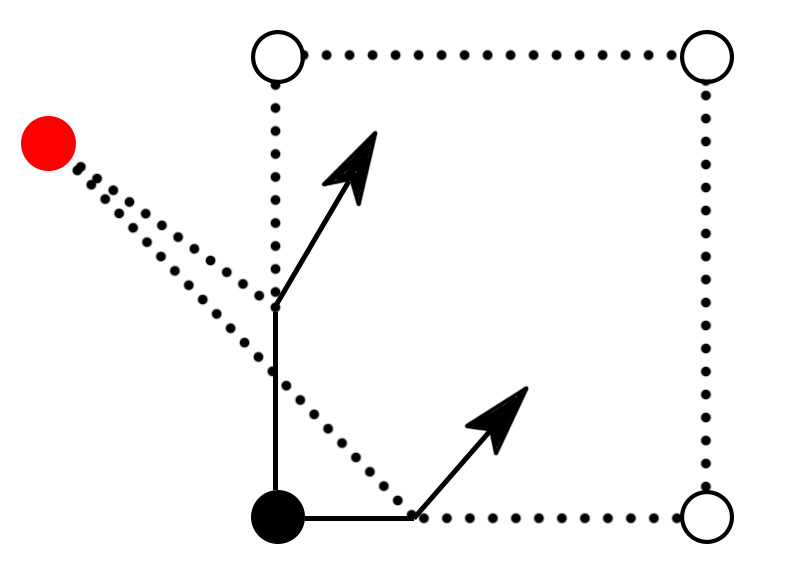
\includegraphics[width=0.4\textwidth]{Figures/DC-colinear.jpg}
    \decoRule
    \caption{Illustration of the challenge of parallel normals, leading to a QEF minimizer point outside the cell.}(\cite{Boristhebrave_2018})
    \label{fig:DC-colinear}
\end{figure}

\item \textbf{Computational Complexity:} Solving the QEF can be computationally intensive, especially for large datasets. This complexity can introduce latency in real-time applications, making it imperative to optimize the QEF minimization process.

\item \textbf{Accuracy and Precision:} Ensuring that the QEF minimizer point accurately represents the underlying data is crucial. However, noise in the data or inaccuracies in the sampling process can skew the QEF results, leading to suboptimal vertex positions.
\end{itemize}

\section{Approach for Handling Challenges in QEF Minimization}
The Quadratic Error Function minimization process involves several steps, each with its challenges and considerations. This section breaks down each step in detail to provide a comprehensive understanding of the algorithm, elucidating the underlying logic and computational methods. Figure \ref{fig:QEF-Flowchart} presents a flowchart that outlines the algorithmic steps for QEF minimization. The subsequent subsections delve into each step, providing code snippets and detailed explanations to clarify the approach.
\begin{figure}
    \centering
    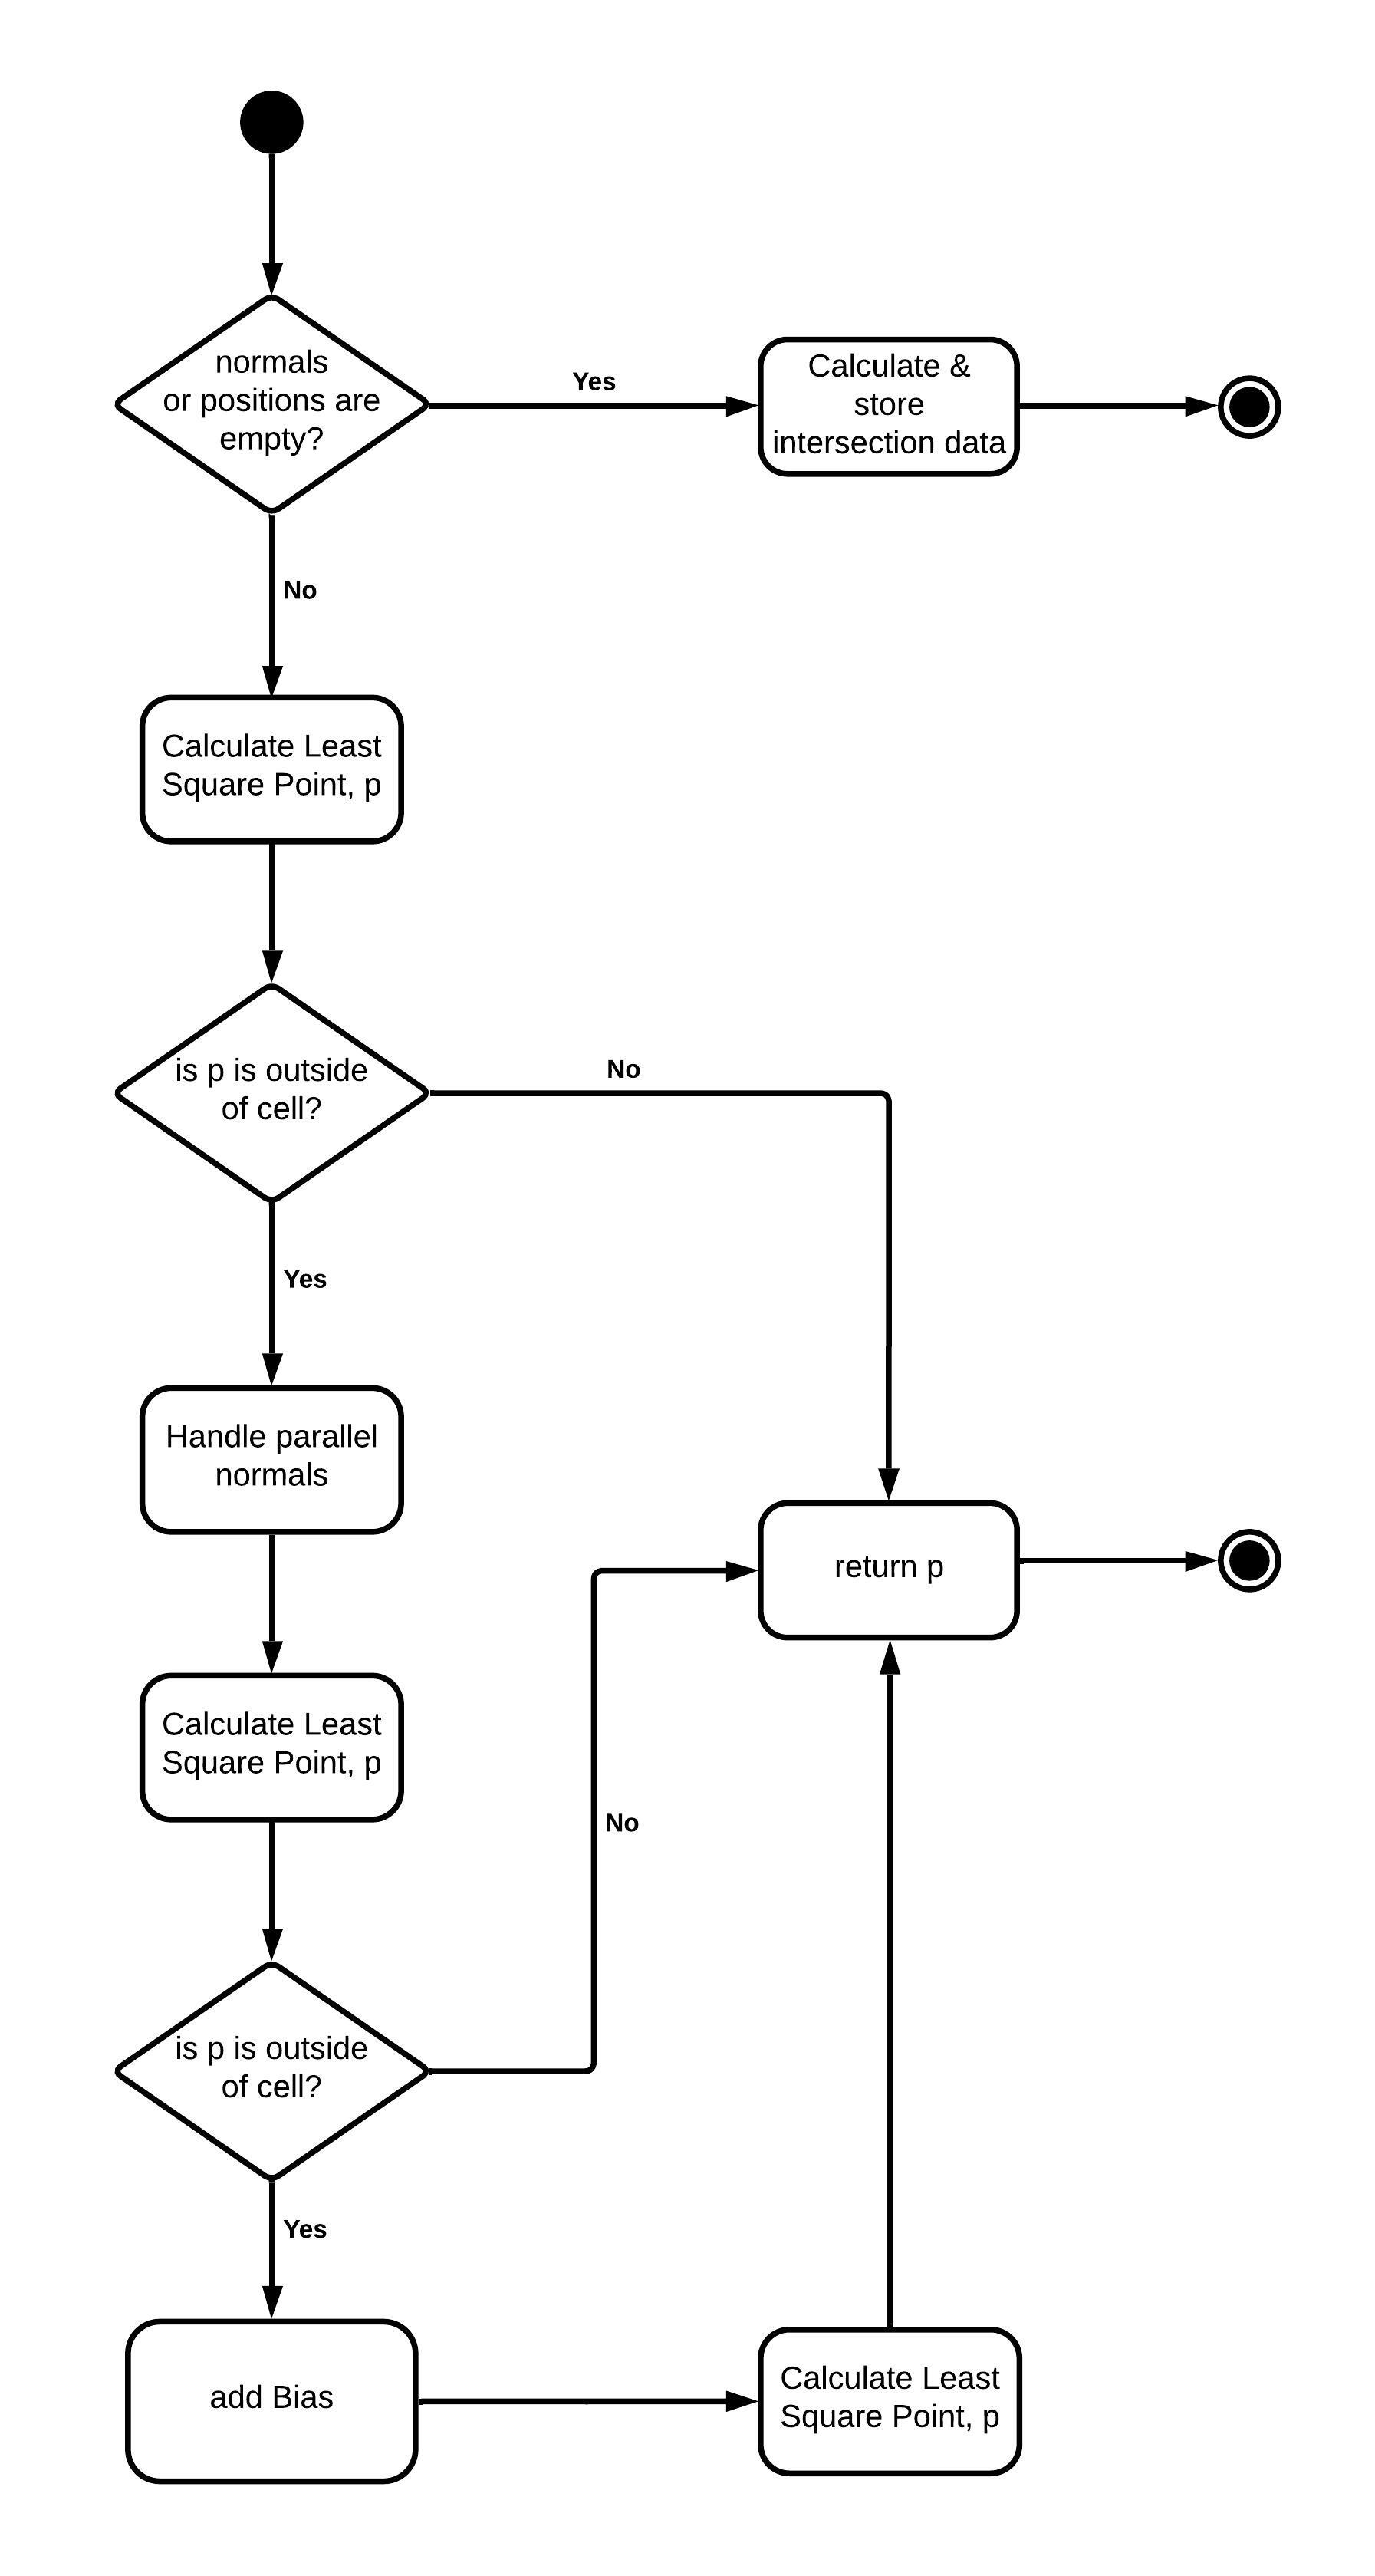
\includegraphics[width=0.83\textwidth]{Figures/QEF-FlowChart.jpeg}
    \decoRule
    \caption{Flowchart illustrating the algorithmic steps involved in QEF minimization for optimal vertex positioning within a cell.}
    \label{fig:QEF-Flowchart}
\end{figure}

\subsection{Check for Empty Normals or Positions}
The algorithm starts by checking if the input vectors for normals or positions are empty. If either is empty, the function returns a zero vector (Listing \ref{lst:isEmpty}).

\vspace{2mm}
\begin{lstlisting}[language=C++, caption=Checking for empty normals or positions, label=lst:isEmpty]
if (normals.empty() || positions.empty())
{
    displayMessage("Invalid data input for QEF calculation. Check your data.\n\n");
    return vector3();  // Return zero vector
}
\end{lstlisting}

\subsection{Initial Least Square Point Calculation}
If the normals and positions are not empty, the algorithm proceeds to calculate the least square point \( p \) using the Tikhonov regularization parameter \( \alpha \) (Listing \ref{lst:callLeastSquarePoint}).

\vspace{2mm}
\begin{lstlisting}[language=C++, caption=Initial least square point calculation, label=lst:callLeastSquarePoint]
// Tikhonov regularization parameter
double alpha = 0.1;

// Calculate the least square point using the previously explained getLeastSquarePoint function (See Listing 5.1)
vector3 p = getLeastSquarePoint(normals, positions, averagePoint, alpha);
\end{lstlisting}

\subsection{Check if Point is Outside the Cell}
The algorithm then checks if the calculated point \( p \) lies outside the cell boundaries using the `isPointOutsideCell` function (Listing \ref{lst:isPointOutside}).

\vspace{2mm}
\begin{lstlisting}[language=C++, caption=Checking if point is outside the cell, label=lst:isPointOutside]
// Check if the point is outside the cell boundaries
bool isPointOutsideCell(const vector3& p, const vector3& cellMinPoint, const vector3& cellMaxPoint)
{
    // Compare the X, Y, and Z coordinates of the point with the minimum and maximum coordinates of the cell
    // A small epsilon (1e-4) is used for tolerance
    return (p.getX() < (cellMinPoint.getX() - 1e-4)) || (point.getX() > (cellMaxPoint.getX() + 1e-4))
        || (p.getY() < (cellMinPoint.getY() - 1e-4)) || (point.getY() > (cellMaxPoint.getY() + 1e-4))
        || (p.getZ() < (cellMinPoint.getZ() - 1e-4)) || (point.getZ() > (cellMaxPoint.getZ() + 1e-4));
}
if (isPointOutside)
{
    // Handle parallel normals in the next step
}
\end{lstlisting}

\subsection{Handling Parallel Normals}
One of the challenges in QEF minimization is the presence of parallel or nearly parallel normals. These can lead to a QEF minimizer point that lies outside the cell. To address this issue, a specialized approach is adopted to detect parallel normals and adjust the QEF calculation accordingly.

The following C++ code snippet \ref{lst:handleParallelNormals} demonstrates the logic for detecting and handling parallel normals:

\vspace{2mm}
\begin{lstlisting}[language=C++, caption=Logic for detecting and handling parallel normals, label=lst:handleParallelNormals]
// Handle parallel or nearly parallel normals and average them
void handleParallelNormals(const std::vector<vector3>& normals, const std::vector<vector3>& positions, std::vector<vector3>& averagedNormals, std::vector<vector3>& averagedPositions)
{
    // Threshold for considering normals as parallel
    const double parallelThreshold = 1e-2;  
    
    // Keep track of which normals have been processed
    std::vector<bool> used(normals.size(), false);  

    // Loop through all normals
    for (int i = 0; i < normals.size(); ++i)
    {
        // Skip if this normal has already been processed
        if (used[i]) continue;  

        vector3 sumNormals = normals[i];
        vector3 sumPositions = positions[i];
        int count = 1;

        // Check for parallel normals
        for (int j = i + 1; j < normals.size(); ++j)
        {
            double dotProduct = normals[i].dot(normals[j]);
            if (!used[j] && dotProduct > (1.0 - parallelThreshold))
            {
                sumNormals = sumNormals + normals[j];
                sumPositions = sumPositions + positions[j];
                count++;
                used[j] = true;
            }
        }

        // Average the parallel normals and positions
        sumNormals.normalize();
        sumPositions /= static_cast<float>(count);

        averagedNormals.push_back(sumNormals);
        averagedPositions.push_back(sumPositions);
    }
}
\end{lstlisting}

In this code, the variable \texttt{parallelThreshold} defines how close the dot product of two normals must be to consider them parallel. The normals are considered parallel if the dot product is greater than \(1.0 - \texttt{parallelThreshold}\). This thresholding is pivotal in determining the alignment of normals. Once identified as parallel, the normals and positions are averaged. This averaging process is foundational in refining the Quadratic Error Function representation. As illustrated in Fig. \ref{fig:QEF-Handling-parallel-normals}, the initial position of the point, before averaging, might not be the optimal solution to the QEF, leading to potential inaccuracies in the surface representation.

However, after the averaging process, the QEF is recalculated. This results in a new point that, as depicted in the figure, is now inside the cell. This new QEF solution point is more representative of the underlying surface, ensuring a closer alignment with the actual data. It's a testament to the power of the averaging process, which not only refines the position of the point but also optimizes the QEF solution, leading to a more accurate and robust surface representation.


\begin{figure}
\centering
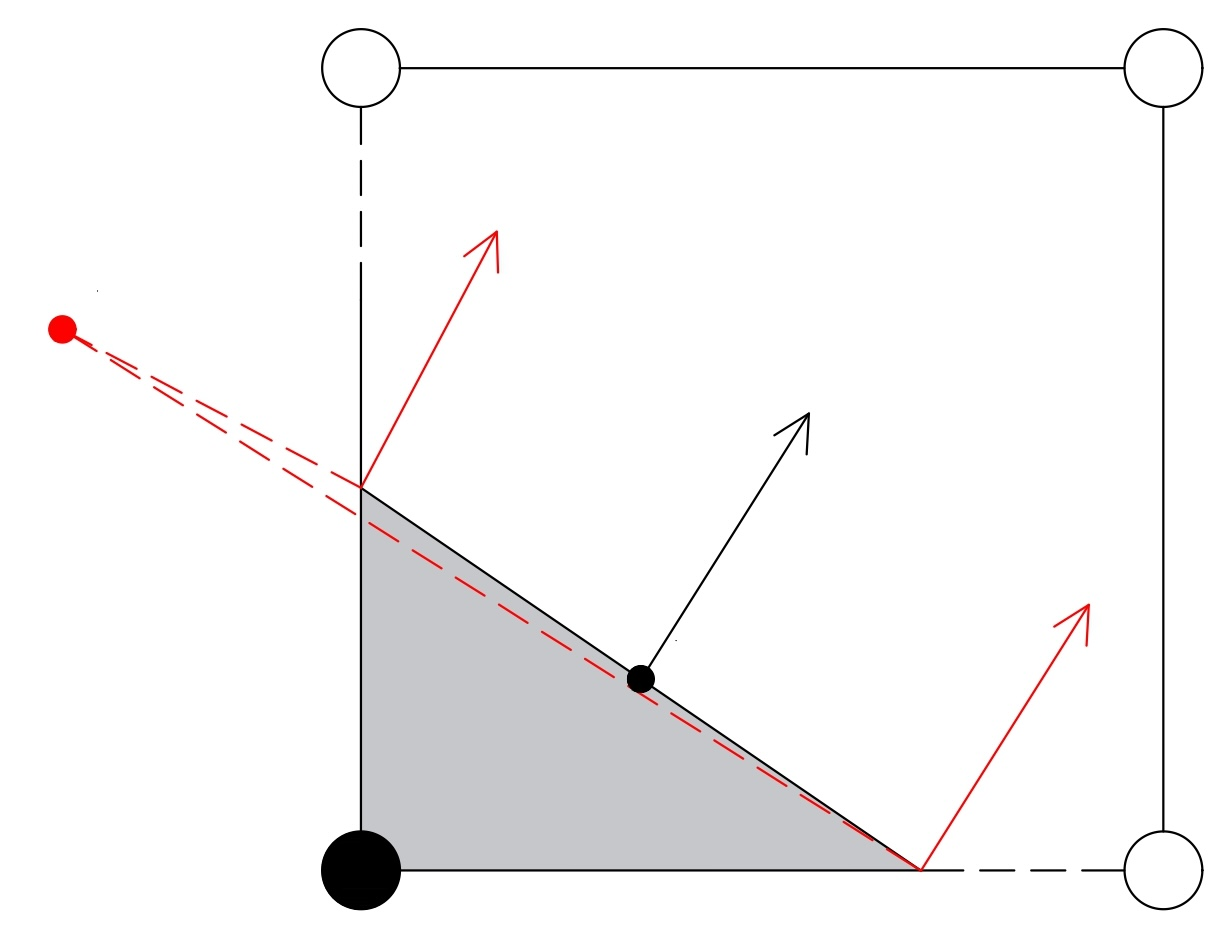
\includegraphics[width=0.6\textwidth]{Figures/aveg-parallal-normals.jpg}
\decoRule
\caption{Illustration of the QEF point refinement process. The red arrows indicate the original normals, representing the initial orientations before refinement. The red point denotes the original QEF solution without handling parallel normals. After addressing and averaging parallel normals, the QEF point is recalculated and represented by the black point. This figure underscores the significance of handling parallel normals in achieving a more accurate surface representation.}
\label{fig:QEF-Handling-parallel-normals}
\end{figure}

\subsection{Adding Bias to Pull Point Towards Cell Center}
If the point \( p \) still lies outside the cell boundaries after handling parallel normals, a bias is added at the center of the cell to pull the QEF point towards the center. This is done by adding additional normals and positions to the averaged list (Listing \ref{lst:addBias}).

\vspace{2mm}
\begin{lstlisting}[language=C++, caption=Adding bias to pull point towards cell center, label=lst:addBias]
// Add bias normals and positions to pull the point towards the cell center
vector3 biasNormalX(0.1, 0.0, 0.0);
vector3 biasNormalY(0.0, 0.1, 0.0);
vector3 biasNormalZ(0.0, 0.0, 0.1);

averagedNormals.push_back(biasNormalX);
averagedNormals.push_back(biasNormalY);
averagedNormals.push_back(biasNormalZ);

averagedPositions.push_back(averagePoint);
averagedPositions.push_back(averagePoint);
averagedPositions.push_back(averagePoint);

// Recalculate the least square point after adding bias
p = getLeastSquarePoint(averagedNormals, averagedPositions, averagePoint, alpha);
\end{lstlisting}

\subsection{Final Check and Clamping the Point}

After adding the bias, the algorithm checks again if the point \( p \) lies outside the cell boundaries. If it does, the point is clamped to the nearest edge of the cell using the \texttt{clamp} function (Listing \ref{lst:clamping}).

\vspace{2mm}
\begin{lstlisting}[language=C++, caption=Final check and clamping the point to the nearest boundary, label=lst:clamping]
// Final check for point outside the cell boundaries
bool isPointOutsideAfterBias = isPointOutsideCell(point, cellMinPoint, cellMaxPoint);

if (isPointOutsideAfterBias)
{
    p.setX(clamp(point.getX(), cellMinPoint.getX(), cellMaxPoint.getX()));
    p.setY(clamp(point.getY(), cellMinPoint.getY(), cellMaxPoint.getY()));
    p.setZ(clamp(point.getZ(), cellMinPoint.getZ(), cellMaxPoint.getZ()));
}
\end{lstlisting}

\subsubsection{Implications of Clamping on Geometric Representation}

The clamping process, while ensuring that the QEF minimizer point lies within the cell, can introduce some geometric artifacts. Specifically, clamping can lead to:

\begin{enumerate}
    \item \textbf{Loss of Surface Smoothness}: When the QEF minimizer point is clamped to the nearest cell boundary, it can disrupt the continuity of the surface, leading to potential sharp edges or corners. This is especially noticeable when multiple adjacent cells have their minimizer points clamped, resulting in a visible discontinuity in the isosurface.
    
    \item \textbf{Deviation from True Surface}: The clamped point might not be the true minimizer of the QEF. As a result, the generated isosurface might deviate from the actual underlying data. This deviation can lead to inaccuracies in the geometric representation, especially in regions with complex surface features.
    
    \item \textbf{Bias towards Cell Boundaries}: The clamping process can introduce a bias where the isosurface tends to adhere more closely to cell boundaries, especially in areas with sparse or ambiguous data. This can lead to an over-representation of the cell grid structure on the final surface.
\end{enumerate}

To address these potential issues, it's essential to strike a balance between ensuring the QEF minimizer point lies within the cell and preserving the integrity of the geometric representation. Some potential solutions include:

\begin{enumerate}
    \item \textbf{Adaptive Cell Sizing with Octree Implementation}: Leveraging octree data structures can facilitate adaptive cell sizing based on the density or complexity of the data. In regions with intricate surface features, the octree can subdivide cells to create smaller cells, leading to a more accurate QEF solution and reducing the need for clamping. The hierarchical nature of the octree ensures efficient spatial subdivision, allowing for finer granularity where needed while maintaining larger cells in less complex regions.
    
    \item \textbf{Post-Processing Smoothing}: After the isosurface generation, a post-processing step can be applied to smooth out the surface, especially in regions affected by clamping. This can help in restoring some of the surface continuity.
\end{enumerate}

\noindent In essence, while clamping offers a practical solution, it's vital to understand its geometric implications and employ strategies to address them for a more accurate isosurface representation. The algorithm effectively handles various challenges in QEF minimization, including empty normals, parallel normals, and points outside the cell boundaries. By adding a bias towards the cell center, the algorithm ensures that the QEF minimizer point is more likely to lie within the cell, thereby improving the accuracy of the generated isosurface.

\section{Code Deployment} 
GitHub (\cite{github}) is a popular desktop and web hosting platform for Continuous Integration (CI) and Continuous Deployment (CD) of software code. The code base of the Simulation Platform is developed on Visual Studio code IDE (Integrated Development Environment). The entire code base and the results of this thesis work are deployed to GitHub and can be viewed via link \url{https://github.com/pth68/SimulationPlatform}.

\section{Summary}
This chapter provided a deep dive into the Quadratic Error Function and its pivotal role in Dual Contouring and Dual Marching Cubes algorithms. The chapter began with simplifying the QEF equation, making it more accessible, and setting the stage for its practical implementation.

The Eigen C++ library emerged as a powerful ally in this journey, enabling efficient and accurate linear algebra operations. The chapter presented a comprehensive algorithmic flow for QEF calculation, addressing challenges such as handling colinear normals and ensuring the calculated point remains within the cell boundaries.

Special attention was given to the challenges in QEF minimization. Strategies like averaging parallel normals and adding a bias towards the cell center were introduced to address potential pitfalls. The chapter also provided a detailed breakdown of the algorithm's steps, from initial checks to the final clamping of the point.

In essence, Chapter \ref{Chapter5} served as a deep dive into the QEF methodology, offering a mix of theory, practical challenges, and coding insights. With a robust understanding of the QEF and its intricacies, readers are well-equipped to tackle the challenges of isosurface extraction. With a solid understanding of QEF methodology and its challenges, the stage is set for us to delve into the practical implementation of the Dual Contouring and Dual Marching Cubes algorithms, which will be the focus of the next chapter.

% \section{Summary}
% This chapter provides a comprehensive overview of the Quadratic Error Function and its application in isosurface extraction, specifically in the context of Dual Contouring and Dual Marching Cubes algorithms. The chapter begins by simplifying the QEF equation and introducing a matrix formulation that is numerically stable and robust, thanks to the application of Singular Value Decomposition and Tikhonov regularization.

% The Eigen C++ library is introduced as a powerful tool for performing the required linear algebra operations efficiently. An algorithmic flow for QEF calculation is presented, complete with a C++ implementation that leverages Eigen's capabilities. The algorithm addresses challenges such as handling colinear normals, computational complexity, and ensuring accuracy and precision.

% Special attention is given to the challenges in QEF minimization, including handling parallel or nearly parallel normals, which can cause the QEF minimizer point to lie outside the cell. The algorithm incorporates checks and balances at multiple stages to ensure the calculated point is within the cell boundaries. If the point lies outside, the algorithm employs strategies like averaging parallel normals and adding a bias towards the cell center to pull the point back into the cell.

% The chapter concludes with a detailed algorithmic flow, breaking down each step involved in QEF minimization. This includes initial checks for empty data, least square point calculation, and specialized handling for parallel normals and points outside the cell.

% Overall, this chapter serves as a comprehensive guide for anyone looking to understand or implement QEF minimization in the context of isosurface extraction. It offers a balanced mix of theory, practical challenges, and coding insights, making it a valuable resource for researchers and practitioners. With a solid understanding of QEF methodology and its challenges, the stage is set for us to delve into the practical implementation of the Dual Contouring and Dual Marching Cubes algorithms, which will be the focus of the next chapter.